\chapter{Zeichnungen}
	\begin{figure}[h]
		\centering
		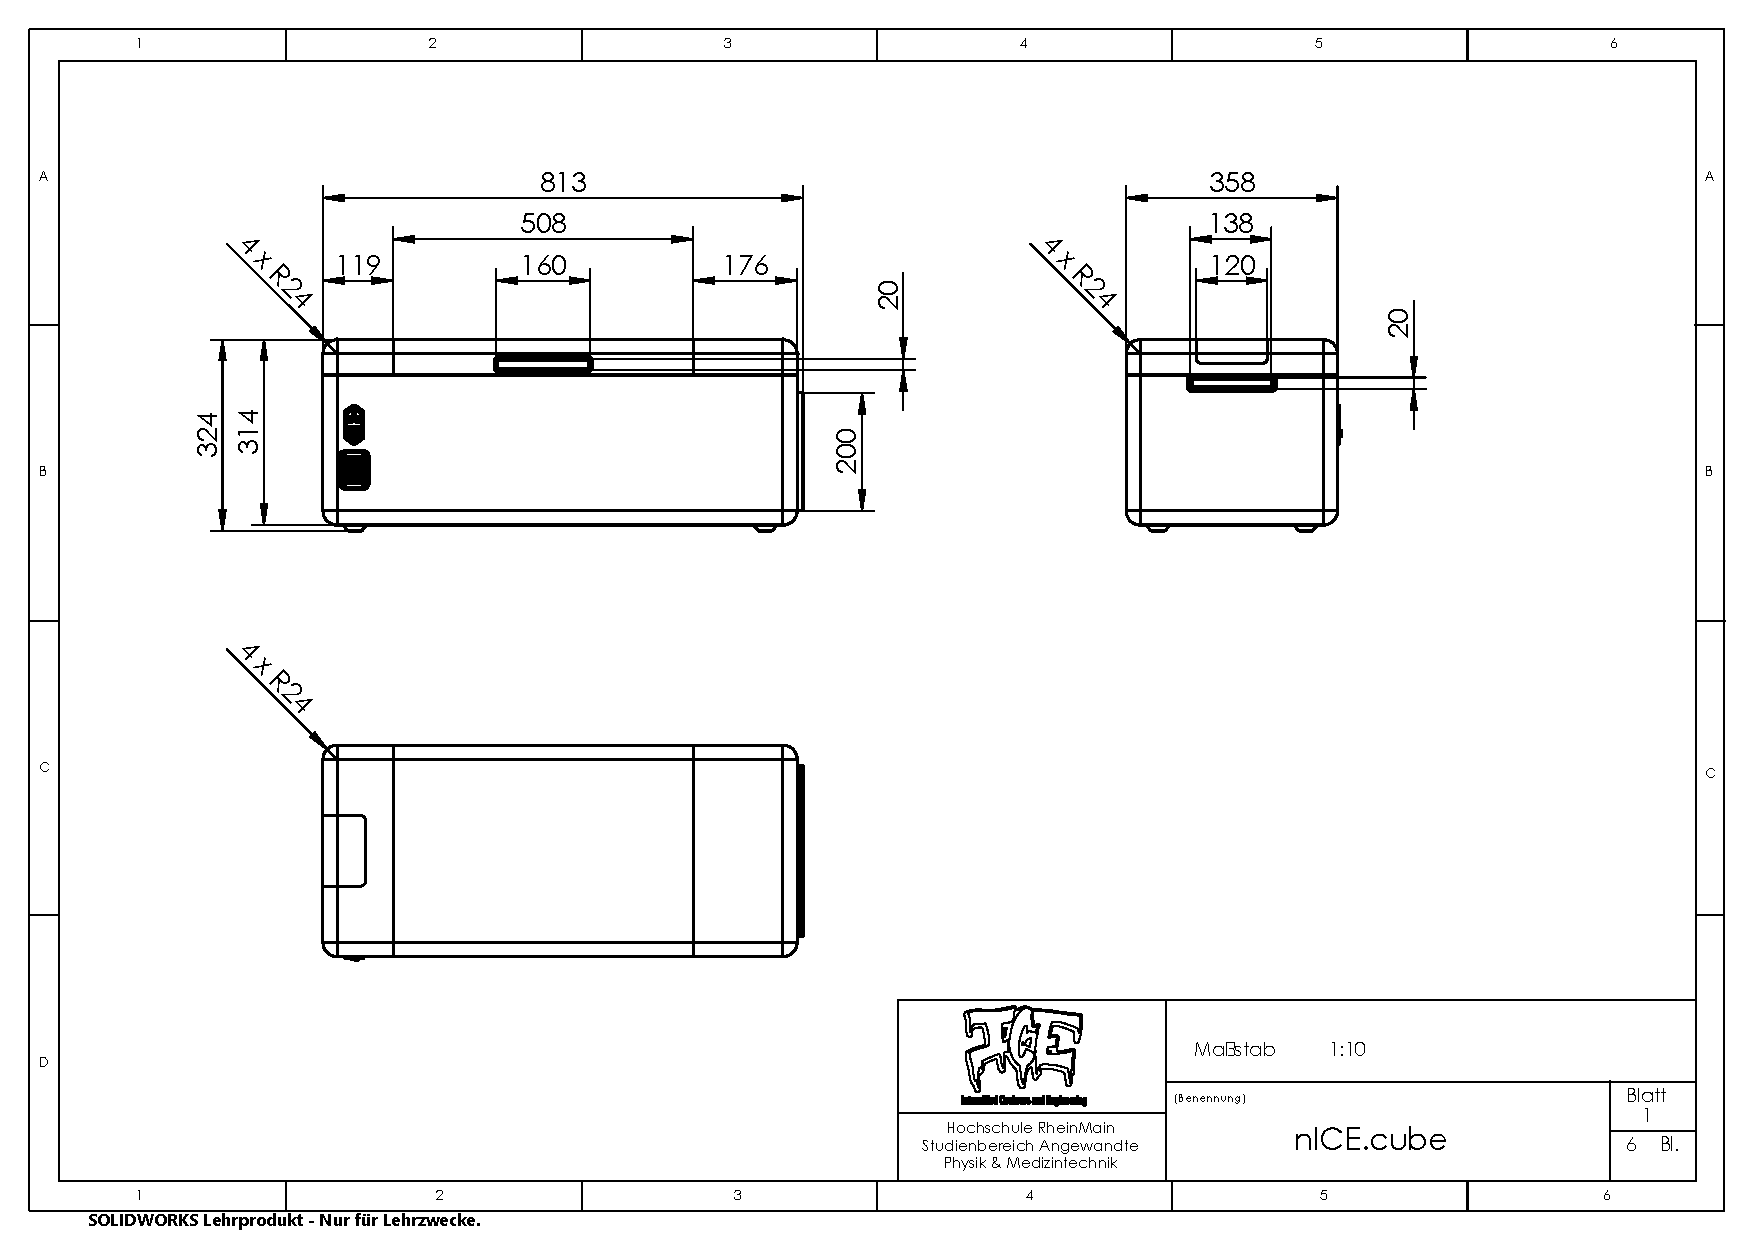
\includegraphics[angle=90, height=\textheight]{Assembly/aussen_zeichnung.PDF}
		\caption[Äußere Dimensionen]{Äußere Dimensionen des \textit{nICE.cube}.}
		\label{fig:zeichnung aussen}
	\end{figure}
	\clearpage
	\begin{figure}[h]
		\centering
		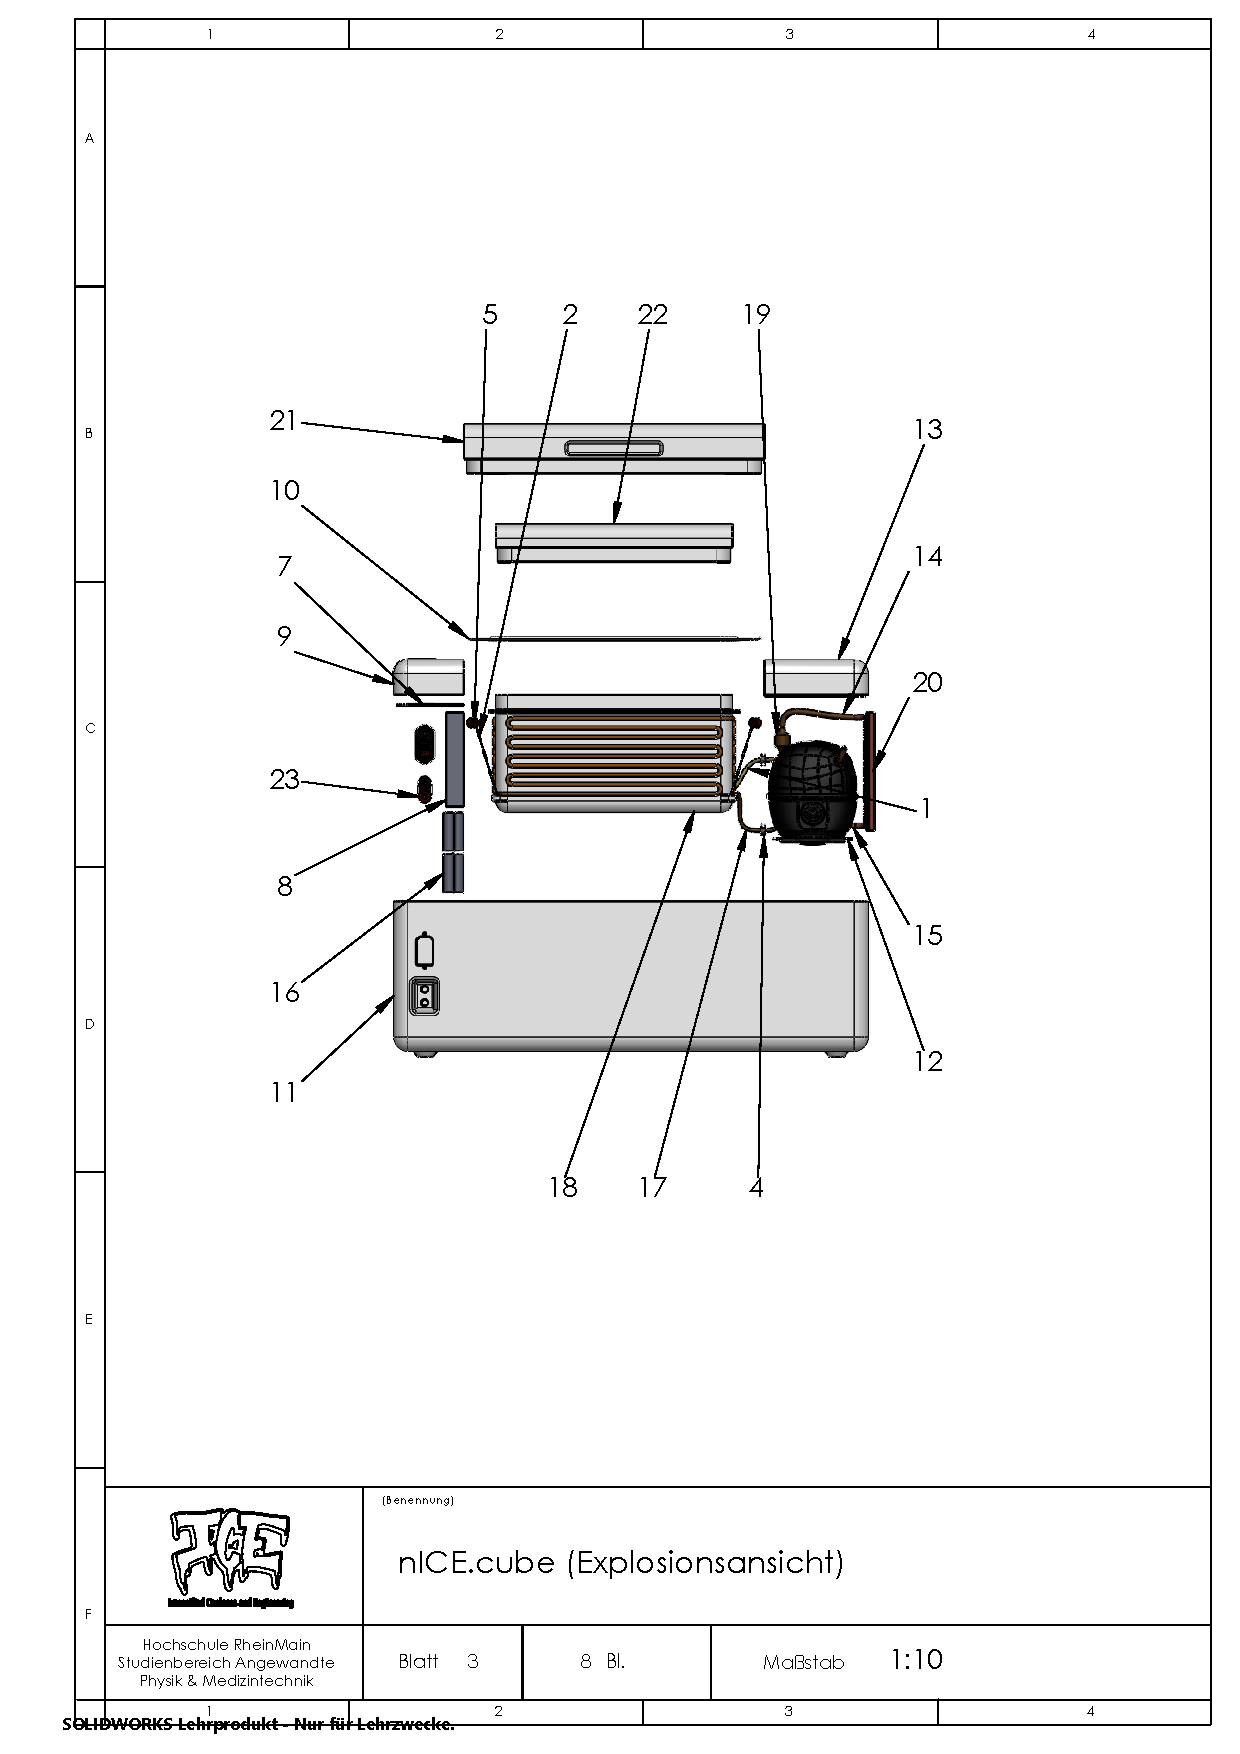
\includegraphics[height=\textheight]{Assembly/explo_zeichnung.PDF}
		\caption[Explosionsansicht]{Explosionsansicht und Positionsnummern der Kernkomponenten.}
		\label{fig:explo}
	\end{figure}
	\clearpage
	\begin{figure}[h]
		\centering
		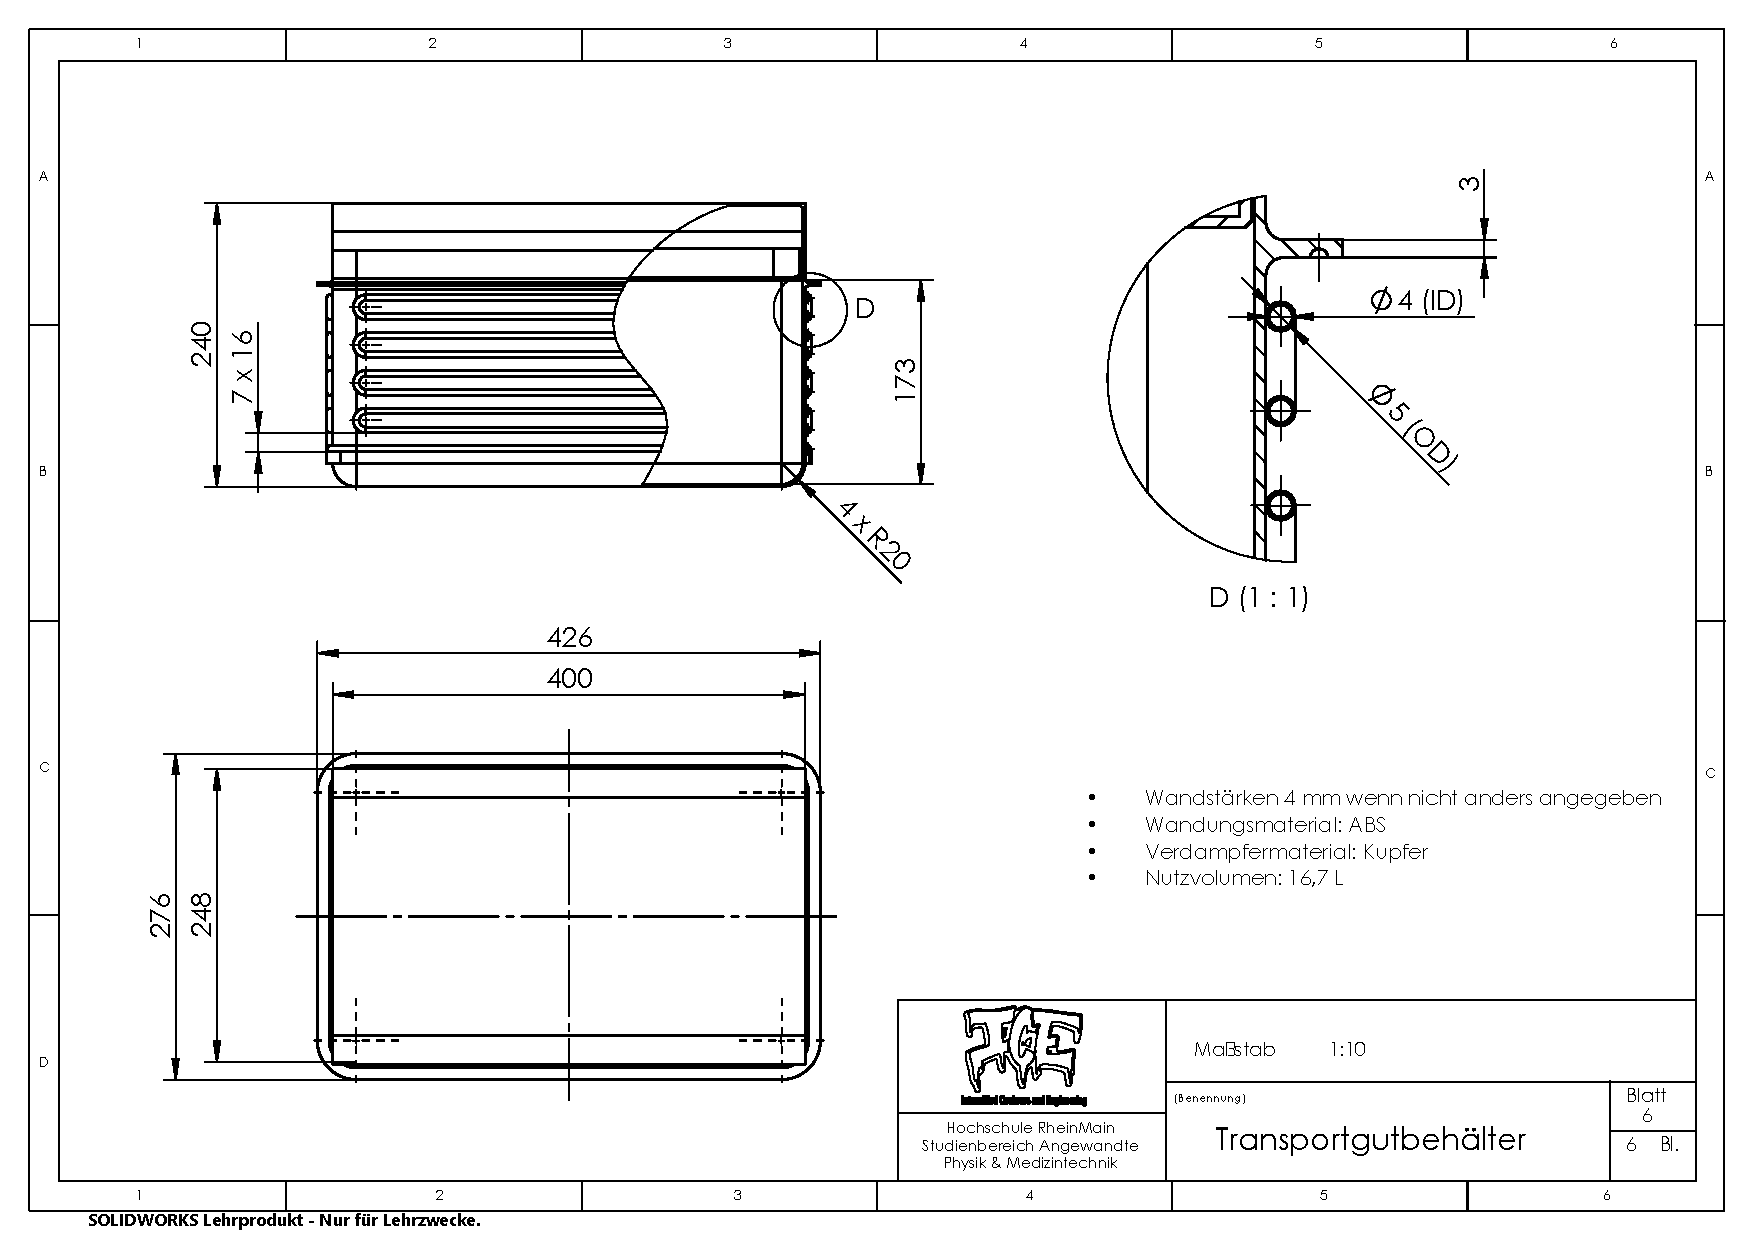
\includegraphics[angle=90, height=\textheight]{Assembly/nutzvolumen_zeichnung.PDF}
		\caption[Detailzeichnung des Kühlbehälters.]{Detailzeichnung des Kühlbehälters.}
		\label{fig:nutzvolumen zeichnung}
	\end{figure}